\documentclass[10pt,a4paper]{article}

\usepackage[margin=0.75cm]{geometry}
\usepackage[utf8]{inputenc}

\usepackage{amsmath}
\usepackage{amssymb}
\usepackage{biblatex}
\usepackage{textcomp}
\usepackage{gensymb}
\usepackage{paracol}
\usepackage{parskip}
\usepackage{tikz}
\usepackage{titlesec}
\usepackage{verbatim}
\usepackage{xcolor}

\titleformat{\section}[block]{\Large\bfseries\filcenter\color{black}}{\thesection}{1em}{}
\titleformat{\subsection}[block]{\bfseries\filcenter\color{black}}{\thesubsection}{1em}{}

\setlength{\columnsep}{25pt}

\tikzset{
    rounded-box/.style = {draw=teal, fill=white, thin, rectangle, rounded corners, inner sep=5pt, inner ysep=10pt},
    rounded-box-title/.style = {fill=teal, text=white, font=\bfseries},
}

\addbibresource{references.bib}

\begin{document}
\title{Discrete Mathematics}

\section{Methods of Proof}

\begin{itemize}
    \item A \textbf{direct proof} proceeds by establishing a chain of implications $P \Rightarrow P_1 \Rightarrow \dots \Rightarrow P_n \Rightarrow Q$ leading directly from $P$ to $Q$. \\

    \item A \textbf{proof by contradiction} assumes that the hypothesis $P$ is true, just as in a direct proof, but then supposes that the conclusion $Q$ is false. \\

    \item Closely related to the method of proof by contradiction is \textbf{proof by contrapositive}: The negative of a statement $P$ is the statement "it is not the case that $P$", abbreviated symbolically as $\neg P$ and pronounced "not $P$".
\end{itemize}

\subsection{Mathematical Induction}

\begin{paracol}{2}

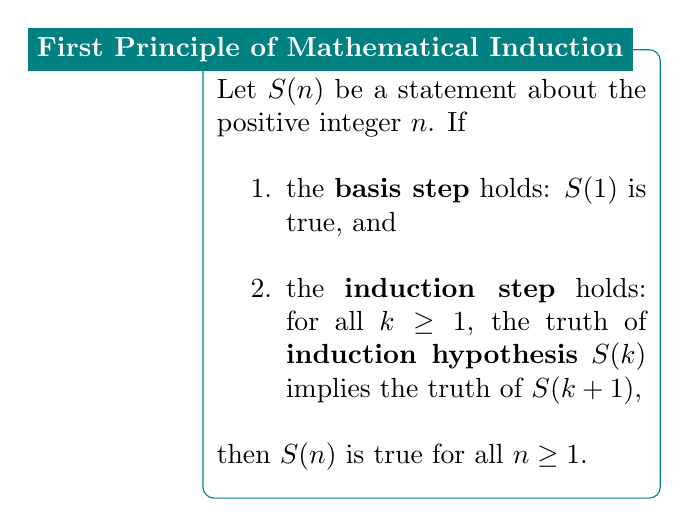
\begin{tikzpicture}
\node [rounded-box] (box){\begin{minipage}{0.45\textwidth}
    Let $S(n)$ be a statement about the positive integer $n$. If \\

    \begin{enumerate}
        \item the \textbf{basis step} holds: $S(1)$ is true, and \\
        \item the \textbf{induction step} holds: for all $k \geq 1$, the truth of \textbf{induction hypothesis} $S(k)$ implies the truth of $S(k+1)$, \\
    \end{enumerate}

    then $S(n)$ is true for all $n \geq 1$.
\end{minipage}};
\node[rounded-box-title, left=10pt] at (box.north east) {First Principle of Mathematical Induction};
\end{tikzpicture}

\switchcolumn

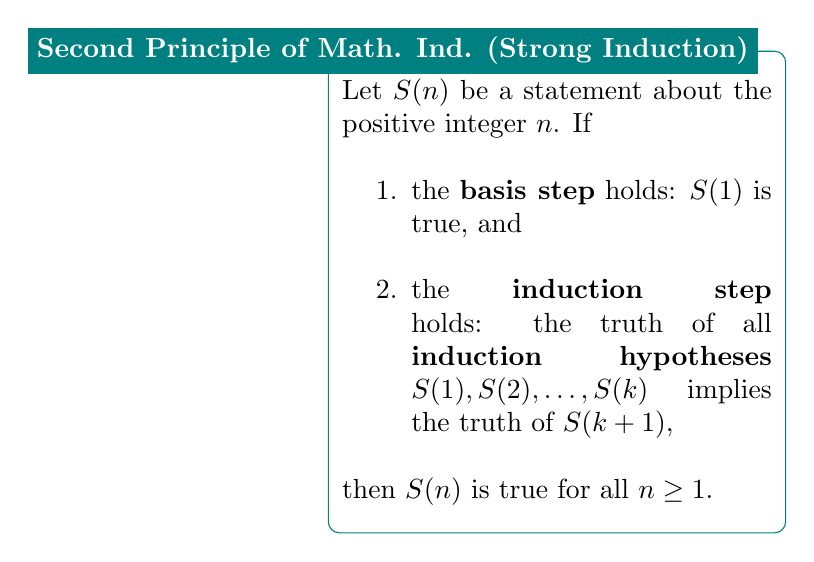
\begin{tikzpicture}
\node [rounded-box] (box){\begin{minipage}{0.45\textwidth}
    Let $S(n)$ be a statement about the positive integer $n$. If \\

    \begin{enumerate}
        \item the \textbf{basis step} holds: $S(1)$ is true, and \\
        \item the \textbf{induction step} holds: the truth of all \textbf{induction hypotheses} $S(1), S(2), \dots, S(k)$ implies the truth of $S(k+1)$, \\
    \end{enumerate}

    then $S(n)$ is true for all $n \geq 1$.
\end{minipage}};
\node[rounded-box-title, left=10pt] at (box.north east) {Second Principle of Math. Ind. (Strong Induction)};
\end{tikzpicture}

\end{paracol}

\section{Combinatorics}

\subsection{Subsection 1}

\begin{paracol}{2}

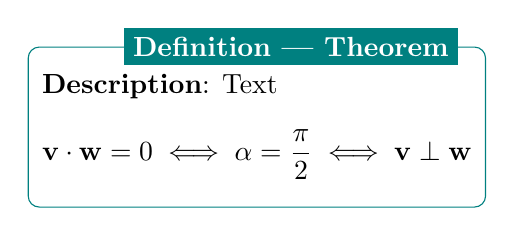
\begin{tikzpicture}
\node [rounded-box] (box){\begin{minipage}{0.45\textwidth}
    \textbf{Description}: Text
    $$\mathbf{v} \cdot \mathbf{w} = 0 \iff \alpha = \frac{\pi}{2} \iff \mathbf{v} \perp \mathbf{w}$$
\end{minipage}};
\node[rounded-box-title, left=10pt] at (box.north east) {Definition | Theorem};
\end{tikzpicture}

\end{paracol}
 \newpage
\section{Asymptotics and Big-O Notation}

\subsection{Subsection 1}

\begin{paracol}{2}

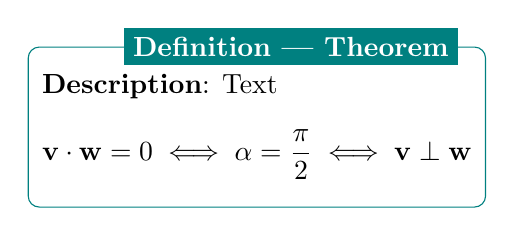
\begin{tikzpicture}
\node [rounded-box] (box){\begin{minipage}{0.45\textwidth}
    \textbf{Description}: Text
    $$\mathbf{v} \cdot \mathbf{w} = 0 \iff \alpha = \frac{\pi}{2} \iff \mathbf{v} \perp \mathbf{w}$$
\end{minipage}};
\node[rounded-box-title, left=10pt] at (box.north east) {Definition | Theorem};
\end{tikzpicture}

\end{paracol}
 \newpage
\section{Graphs}

\subsection{Subsection 1}

\begin{paracol}{2}


\begin{tikzpicture}
\node [rounded-box] (box){\begin{minipage}{0.45\textwidth}
    \textbf{Isomorphic}:
\end{minipage}};
\node[rounded-box-title, left=10pt] at (box.north east) {Definition};
\end{tikzpicture}

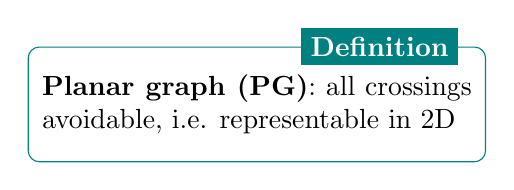
\begin{tikzpicture}
\node [rounded-box] (box){\begin{minipage}{0.45\textwidth}
    \textbf{Planar graph (PG)}: all crossings avoidable, i.e. representable in 2D
\end{minipage}};
\node[rounded-box-title, left=10pt] at (box.north east) {Definition};
\end{tikzpicture}

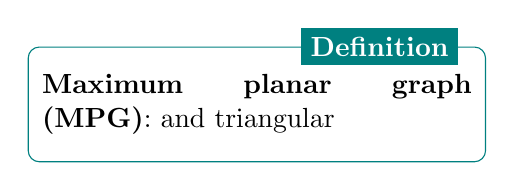
\begin{tikzpicture}
\node [rounded-box] (box){\begin{minipage}{0.45\textwidth}
    \textbf{Maximum planar graph (MPG)}: and triangular
\end{minipage}};
\node[rounded-box-title, left=10pt] at (box.north east) {Definition};
\end{tikzpicture}

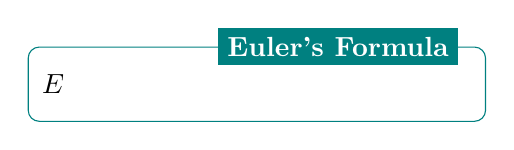
\begin{tikzpicture}
\node [rounded-box] (box){\begin{minipage}{0.45\textwidth}
    $E$
\end{minipage}};
\node[rounded-box-title, left=10pt] at (box.north east) {Euler's Formula};
\end{tikzpicture}

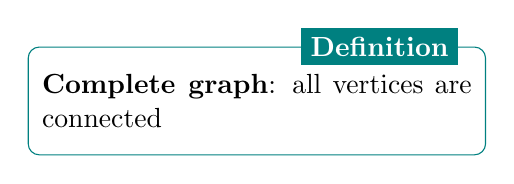
\begin{tikzpicture}
\node [rounded-box] (box){\begin{minipage}{0.45\textwidth}
    \textbf{Complete graph}: all vertices are connected
\end{minipage}};
\node[rounded-box-title, left=10pt] at (box.north east) {Definition};
\end{tikzpicture}

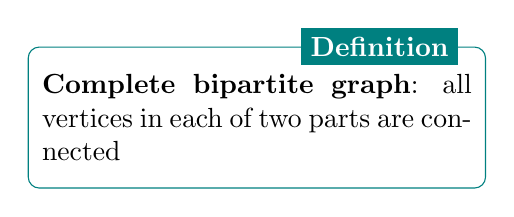
\begin{tikzpicture}
\node [rounded-box] (box){\begin{minipage}{0.45\textwidth}
    \textbf{Complete bipartite graph}: all vertices in each of two parts are connected
\end{minipage}};
\node[rounded-box-title, left=10pt] at (box.north east) {Definition};
\end{tikzpicture}

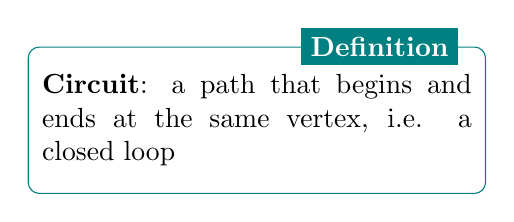
\begin{tikzpicture}
\node [rounded-box] (box){\begin{minipage}{0.45\textwidth}
    \textbf{Circuit}: a path that begins and ends at the same vertex, i.e. a closed loop
\end{minipage}};
\node[rounded-box-title, left=10pt] at (box.north east) {Definition};
\end{tikzpicture}

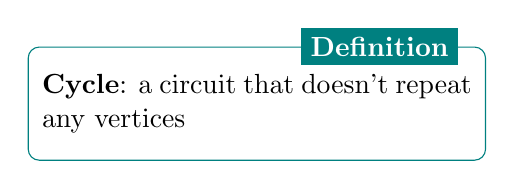
\begin{tikzpicture}
\node [rounded-box] (box){\begin{minipage}{0.45\textwidth}
    \textbf{Cycle}: a circuit that doesn't repeat any vertices
\end{minipage}};
\node[rounded-box-title, left=10pt] at (box.north east) {Definition};
\end{tikzpicture}

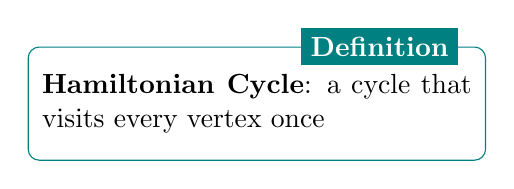
\begin{tikzpicture}
\node [rounded-box] (box){\begin{minipage}{0.45\textwidth}
    \textbf{Hamiltonian Cycle}: a cycle that visits every vertex once
\end{minipage}};
\node[rounded-box-title, left=10pt] at (box.north east) {Definition};
\end{tikzpicture}

Many (but not all) MPGs have a HC.

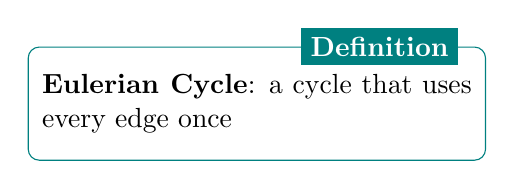
\begin{tikzpicture}
\node [rounded-box] (box){\begin{minipage}{0.45\textwidth}
    \textbf{Eulerian Cycle}: a cycle that uses every edge once
\end{minipage}};
\node[rounded-box-title, left=10pt] at (box.north east) {Definition};
\end{tikzpicture}

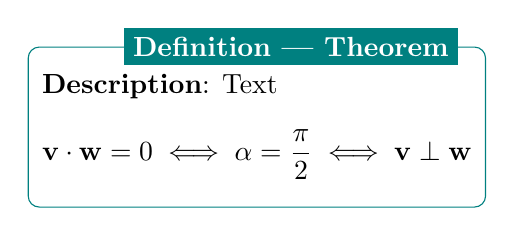
\begin{tikzpicture}
\node [rounded-box] (box){\begin{minipage}{0.45\textwidth}
    \textbf{Description}: Text
    $$\mathbf{v} \cdot \mathbf{w} = 0 \iff \alpha = \frac{\pi}{2} \iff \mathbf{v} \perp \mathbf{w}$$
\end{minipage}};
\node[rounded-box-title, left=10pt] at (box.north east) {Definition | Theorem};
\end{tikzpicture}

\end{paracol}
 \newpage
\section{Connectivity, Trees, Cycles}

\subsection{Subsection 1}

\begin{paracol}{2}

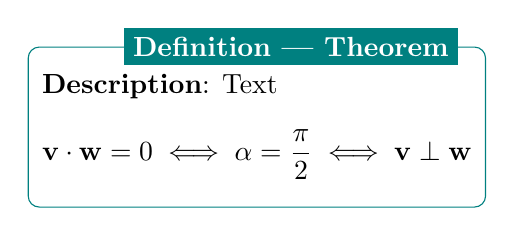
\begin{tikzpicture}
\node [rounded-box] (box){\begin{minipage}{0.45\textwidth}
    \textbf{Description}: Text
    $$\mathbf{v} \cdot \mathbf{w} = 0 \iff \alpha = \frac{\pi}{2} \iff \mathbf{v} \perp \mathbf{w}$$
\end{minipage}};
\node[rounded-box-title, left=10pt] at (box.north east) {Definition | Theorem};
\end{tikzpicture}

\end{paracol}
 \newpage
\section{Eulerian and Hamiltonian Cycles}

\subsection{Subsection 1}

\begin{paracol}{2}

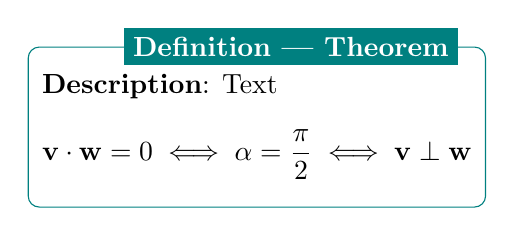
\begin{tikzpicture}
\node [rounded-box] (box){\begin{minipage}{0.45\textwidth}
    \textbf{Description}: Text
    $$\mathbf{v} \cdot \mathbf{w} = 0 \iff \alpha = \frac{\pi}{2} \iff \mathbf{v} \perp \mathbf{w}$$
\end{minipage}};
\node[rounded-box-title, left=10pt] at (box.north east) {Definition | Theorem};
\end{tikzpicture}

\end{paracol}
 \newpage
\section{Spanning Trees}

\subsection{Subsection 1}

\begin{paracol}{2}

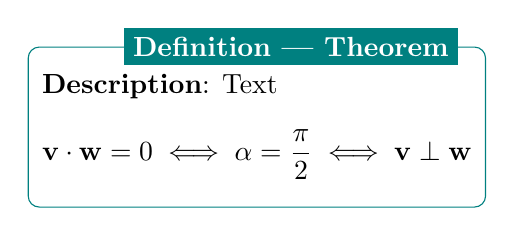
\begin{tikzpicture}
\node [rounded-box] (box){\begin{minipage}{0.45\textwidth}
    \textbf{Description}: Text
    $$\mathbf{v} \cdot \mathbf{w} = 0 \iff \alpha = \frac{\pi}{2} \iff \mathbf{v} \perp \mathbf{w}$$
\end{minipage}};
\node[rounded-box-title, left=10pt] at (box.north east) {Definition | Theorem};
\end{tikzpicture}

\end{paracol}
 \newpage
\section{Maximum Flow and Minimum Cut}

\subsection{Subsection 1}

\begin{paracol}{2}

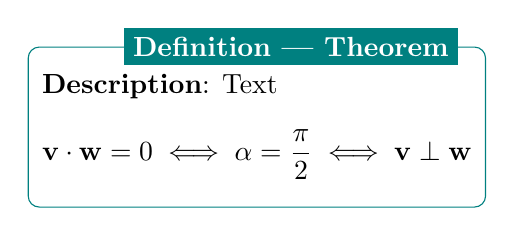
\begin{tikzpicture}
\node [rounded-box] (box){\begin{minipage}{0.45\textwidth}
    \textbf{Description}: Text
    $$\mathbf{v} \cdot \mathbf{w} = 0 \iff \alpha = \frac{\pi}{2} \iff \mathbf{v} \perp \mathbf{w}$$
\end{minipage}};
\node[rounded-box-title, left=10pt] at (box.north east) {Definition | Theorem};
\end{tikzpicture}

\end{paracol}
 \newpage
\section{Matchings in Bipartite Graphs}

\subsection{Subsection 1}

\begin{paracol}{2}

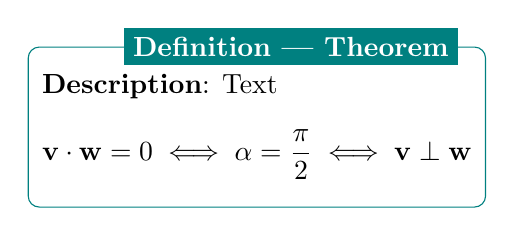
\begin{tikzpicture}
\node [rounded-box] (box){\begin{minipage}{0.45\textwidth}
    \textbf{Description}: Text
    $$\mathbf{v} \cdot \mathbf{w} = 0 \iff \alpha = \frac{\pi}{2} \iff \mathbf{v} \perp \mathbf{w}$$
\end{minipage}};
\node[rounded-box-title, left=10pt] at (box.north east) {Definition | Theorem};
\end{tikzpicture}

\end{paracol}
 \newpage

\nocite{*}
\printbibliography

\end{document}
